\documentclass[ngerman]{fbi-aufgabenblatt}

\usepackage{amsmath}
\usepackage{amssymb}
\usepackage{verbatim}
\usepackage{tikz}

% Folgende Angaben bitte anpassen

\renewcommand{\Vorlesung}{Grundlagen der Wissensverarbeitung}
\renewcommand{\Semester}{WiSe 17/18}

\renewcommand{\Aufgabenblatt}{9}
\renewcommand{\Teilnehmer}{ Übungsgruppe 2; Tom Kastek (4kastek@inf), Phil Sehlmeyer (4sehlmey@inf), Max Wutz (wutzmax@googlemail.com)}

\begin{document}

\aufgabe{Exercise 9.2: (Language Modelling)}

Unser Programm wirft nur aneinandergereihte Worte aus. So machen zwar meistens die Worte Sinn, die auf ein Wort folgen, aber ein entstehender Satz macht am Ende keinen Sinn mehr. Also sind Gemeinsamkeiten nur darin zu erkennen, dass man die Worte erkennt und man sich vorstellen kann, wie aus zwei Worten ein Satz gebaut werden könnte. Aber alles darüber hinaus ist komplett unterschiedlich und im Realen nicht mehr verständlich.

\aufgabe{Exercise 9.3: (Diagnosis (cont.))}

Belief Network\\

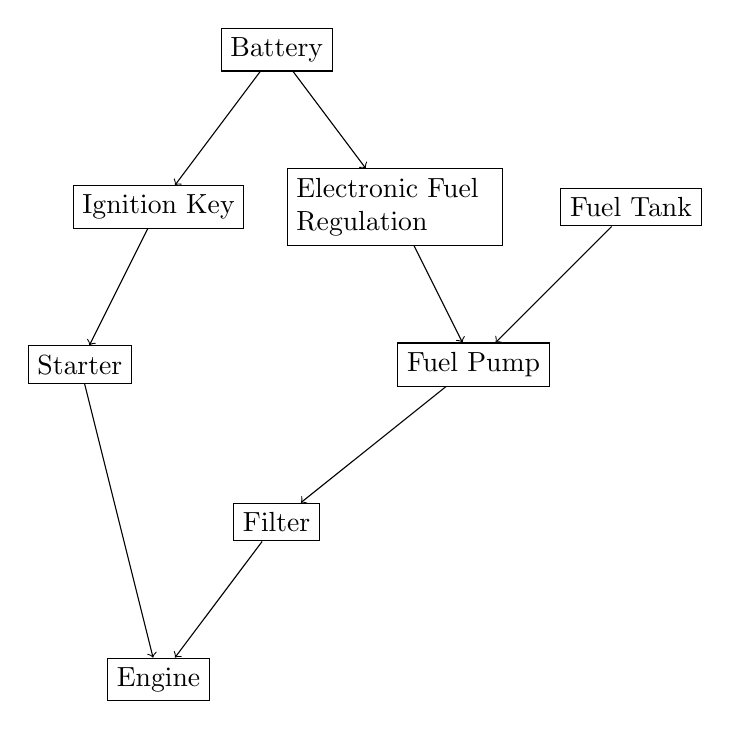
\begin{tikzpicture}
	\node [shape=rectangle,draw=black] (E) at (-1.5,-4) {Engine};
	\node [shape=rectangle,draw=black] (S) at (-2.5,0) {Starter};
	\node [shape=rectangle,draw=black] (F) at (0,-2) {Filter};
	\node [shape=rectangle,draw=black] (FP) at (2.5,0) {Fuel Pump};
	\node [shape=rectangle,draw=black] (FT) at (4.5,2) {Fuel Tank};
	\node [shape=rectangle,draw=black] (I) at (-1.5,2) {Ignition Key};
	\node [text width=2.5cm,shape=rectangle,draw=black] (EFR) at (1.5,2) {Electronic Fuel Regulation};
	\node [shape=rectangle,draw=black] (B) at (0,4) {Battery};
	
	\path [->] (B) edge node {} (I);
	\path [->] (B) edge node {} (EFR);
	\path [->] (I) edge node {} (S);
	\path [->] (S) edge node {} (E);
	\path [->] (FT) edge node {} (FP);
	\path [->] (FP) edge node {} (F);
	\path [->] (F) edge node {} (E);
	\path [->] (EFR) edge node {} (FP); 
\end{tikzpicture}

Aus der Aufgabenstellung ableitbare Wahrscheinlichkeiten:
\begin{align*}
&P(Battery) &&= 0.9\\
&P(\neg Battery) &&= 0.1\\
&\\
&P(Ignition Key|Battery) &&= 0.9\\
&P(\neg Ignition Key| Battery) &&= 0.1\\
&\\
&P(Electronic Fuel Regulation|Battery) &&= 0.9\\
&P(\neg Electronic Fuel Regulation| Battery) &&= 0.1\\
&\\
&P(Fuel Tank) &&= 0.9\\
&P(\neg Fuel Tank) &&= 0.1\\
&\\
&P(Starter| Ignition Key) &&= 0.9\\
&P(\neg Starter | Ignition Key) &&= 0.1\\
&\\
&P(Fuel Pump | Electronic Fuel Regulation \land Fuel Tank) &&= 0.9\\
&P(\neg Fuel Pump | Electronic Fuel Regulation \land Fuel Tank) &&= 0.1\\
&\\
&P(Filter | Fuel Pump) &&= 0.9\\
&P(\neg Filter | Fuel Pump) &&= 0.1\\
&\\
&P(Engine | Starter \land Filter) &&= 0.9\\
&P(\neg Engine | Starter \land Filter) &&= 0.1\\
\end{align*}

Aufgabenstellungen:

\begin{itemize}
\item Die Wahrscheinlichkeit, dass die Battery funktioniert: Aus den oben angegebenen Wahrscheinlichkeiten ablesbar. \(P(Battery) = 0.9\)
\item Die Wahrscheinlichkeit, dass der Starter funktioniert: Dafür müssen die davor liegenden Teile funktionieren, also der Ignition Key und die Battery. \(P(Battery) \cdot P(IgnitionKey|Battery \cdot P(Starter|IgnitionKey) = 0.9 \cdot 0.9 \cdot 0.9 = 0.729\)
\item Die Wahrscheinlichkeit, dass die Engine funktioniert: Es müssen sämtliche Vorgänger im Netzwerk und die Engine selbst, also alle, funktionieren. \(0.9^{8} \approx 0.430\)
\item Die Wahrscheinlichkeit, dass die Engine funktioniert, gegeben, dass die Pump funktioniert. Da die Pump funktioniert, müssen sämtliche Vorgänger im Network ebenfalls funktionieren, also Electronic Fuel Regulation, Battery, und Fuel Tank. Diese fallen also aus der Rechnung raus. \(0.9^{4} \approx 0.656\)
\end{itemize}


\aufgabe{Exercise 9.4: (Bayesian Probabilities)}

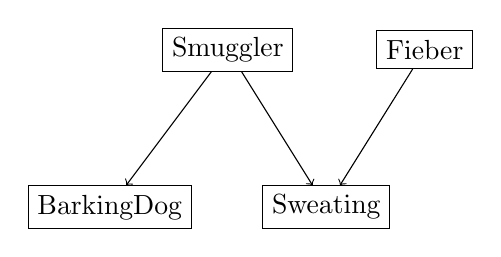
\begin{tikzpicture}
	\node [shape=rectangle,draw=black] (B) at (-1.5,2) {BarkingDog};
	\node [shape=rectangle,draw=black] (F) at (2.5,4) {Fieber};
	\node [shape=rectangle,draw=black] (Sm) at (0,4) {Smuggler};
	\node [shape=rectangle,draw=black] (Sw) at (1.25,2) {Sweating};
	
	\path [->] (Sm) edge node {} (B);
	\path [->] (Sm) edge node {} (Sw);
	\path [->] (F) edge node {} (Sw);
\end{tikzpicture}

\begin{align*}
&P(Smuggler) &&= 0.01\\
&P(\neg Smuggler) &&= 0.99\\
&\\
&P(BarkingDog | Smuggler) &&= 0.8\\
&P(\neg BarkingDog | Smuggler) &&= 0.2\\
&P(BarkingDog | \neg Smuggler) &&= 0.05\\
&P(\neg BarkingDog | \neg Smuggler) &&= 0.95\\
&\\
&P(Sweating | \neg Smuggler \land  \neg Fieber) &&= 0.00\\
&P(Sweating |  Smuggler \land \neg Fieber) &&= 0.4\\
&P(Sweating |  \neg Smuggler \land Fieber) &&= 0.6\\
&P(Sweating |  Smuggler \land Fieber) &&= 0.8\\
&\\
&P(Sweating |  \neg(Smuggler \land Fieber)) &&= 0.2\\
&\\
&P(Fieber) &&= 0.013\\
&P(\neg Fieber) &&= 0.987\\
\end{align*}

Erklärung des Explaining Away-Effekts anhand des Belief Networks: \\
Nehmen wir an, wir beobachten, dass die verdächtigte Person schwitzt. Aus unserem Netzwerk entnehmen wir, dass die Wahrscheinlichkeiten für Smuggler und Fieber steigen, nun, da wir über das Schwitzen wissen. Wenn wir nun auch beobachten, dass der Hund bellt, erhöht dieses Wissen erneut die Wahrscheinlichkeit für Smuggler, vor allem aber deutlicher als für Fieber. Hier sehen wir den Explain away Effekt, durch die Beobachtungen ist Smuggler deutlich wahrscheinlicher als Fieber, Fieber wurde \glqq weg erklärt\grqq{}.

\newpage

Berechnen weiterer Wahrscheinlichkeiten:
\begin{align*}
&P(Smuggler | BarkingDog)\\
\end{align*}
\begin{align*}
&P(Smuggler | BarkingDog) &&= (P(BarkingDog | Smuggler) \cdot P(Smuggler)) / P(BarkingDog) \\
& &&= (0.8 \cdot 0.01) / 0.0575\\
& &&= 0,014\\
&\\
&P(BarkingDog) &&= P(Smuggler) \cdot P(BarkingDog | Smuggler) \\
& &&   + P( \neg Smuggler) \cdot P(BarkingDog | \neg Smuggler) \\
& &&= 0.01 \cdot 0.8 + 0.99 \cdot 0.05 \\
& &&= 0.0575 \\
\end{align*}
\begin{align*}
&P(Sweating)\\
\end{align*}
\begin{align*}
&P(Sweating) &&= P(Smuggler \land Fieber) \cdot  P(Sweating | Smuggler \land Fieber)\\
& && + P(\neg(Smuggler \land Fieber)) \cdot  P(Sweating | \neg(Smuggler \land Fieber)\\
& &&= 0.00013 \cdot 0.8 + 0.99987 \cdot 0.2 \\
& &&= 0.2 \\
&P(Smuggler \land Fieber) &&= 0.01 \cdot 0.013 \\
& &&= 0,00013\\
& P(\neg(Smuggler \land Fieber)) &&= P(\neg Smuggler \land Fieber) + P(\neg Smuggler \land \neg Fieber) \\
& &&+P(Smuggler \land \neg Fieber) \\
& &&= 0.99 \cdot 0.013 + 0.99 \cdot 0.987 + 0.01 \cdot 0.987 \\
& &&= 0,99987
\end{align*}
\begin{align*}
&P(Smuggler | BarkingDog \land Sweating)\\
\end{align*}

\end{document}